\documentclass{article}
\title{Nanotechnology}
\author{Zachariah Sachs (with Jeff Montgomery)}
\usepackage{graphicx}
\usepackage{float}
\usepackage{IEEEtrantools}
\usepackage{textcomp}
\usepackage{fixltx2e}

\begin{document}
\maketitle
\section{Purpose}

In this laboratory exercise, we made several sizes of cadmium selenide nanocrystals an gold 
nanoparticles and then analyzed their spectral properties in solution
in order to observe the novel electronic properties of semiconductors and metals of size
comparable to their excitation wavelengths.

\section{Theory and Methods}

\subsection{Semiconductor energy shift and nanocrystals}

When a semiconductor nanocrystal absorbs a photon of sufficient energy, an 
electron-valence hole
pair is created by the promotion of an electron from the valence band to the conduction band
of the material. This pair maintains a charge separation, the bulk Bohr exciton radius, 
generally the size of the Bohr radius of the electron wavefunction in the material, for CdSe
about 5.6 nm. If the bulk of the material is smaller than the corresponding diameter, the 
electron-hole pair cannot achieve this separation, and becomes trapped as in a quantum 
mechanical particle in a box, with accompanying discretization of energy levels.
Discrete energy levels yield distinct electronic transitions, and thus sharper absorption and
emission spectra. In particular, we are able to resolve a downshift in the transition energy
from absorption to emission. This shift results as the system relaxes towards equilibrium in
reaction to the location of the electron; following absorbtion, the internuclear distance in
the crystal decreases, lowering the attractive coulombic potential energy of the electron-hole 
pair, and following emission, the internuclear distance expands, lowering the repulsive
coulombic potential energy of the nuclei to return to the initial energy.

Assuming a uniform, spherical, singly-excitable particle with no electron probability outside,
the solutions to the Schr\"odinger equation for just the electron gives the energies of a
particle in a box:
\begin{equation}
E_n=\frac{h^2n^2}{8 m_c R^2}, \qquad n=1,2,3,\ldots
\end{equation}
where $h$ is Planck's constant, $m_c$ is the effective mass of the electron, and
$R$ is the radius of the nanocrystal, the boundaries of the box. However, to conserve charge,
we must also include the hole. The Hamiltonian for this 2-particle box has a potential energy
term consisting of a Coulomb term and a polarization term which both depend on the
electron-hole separation. The lowest energy of the system, called an exciton, can be 
approximated assuming no correlation between the electron and hole wavefunctions, i.e.
\begin{equation}
\Phi_{ex}(\hat{S}_{elec},\hat{S}_{hole})=\Psi_1(\hat{S}_{elec})\Psi_1(\hat{S}_{hole}),
\end{equation}
for $\hat{S}_{elec}$ and $\hat{S}_{hole}$ the positions of electron and hole, respectively.
This gives energies
\begin{equation}
E_{ex}=\frac{h^2}{8 R^2}\left(\frac{1}{m_e}+\frac{1}{m_h}\right)
-\frac{1.8 e^2}{4\pi\epsilon_{CdSe}\epsilon_0 R}+E_{pol}(R),
\end{equation}
for $m_e$ and $m_h$ the effective masses of electron and hole, respectively,
$\epsilon_{CdSe}$ the dielectric constant of CdSe, $\epsilon_0$ the permittivity of
vacuum, and $E_{pol}(R)$ the polarization energy which is dominated by the kinetic and
and Coulomb energies.
The energy of the lowest optical transition,
\begin{equation}
E_{np}=E_{ex}+E_g,
\end{equation}
is the sum of the exciton and bulk band
gap energies. This gives an equation which is quadratic in $R$ and can be solved for taking
$E_{np}$ from the peak of the spectral absorption band.

\subsection{Metallic nanoparticles}

Conducting electrons in metallic particles of sizes smaller than excitation wavelengths 
resonate between available states upon absorption of visible light and are called
surface plasmons. Mie theory predicts
the absorbance of a dilute solution of such particles as
\begin{equation}
A=\log_{10}\frac{I}{I_0}=\frac{CNd}{2.303},
\end{equation}
where $C$ is the absorption cross section, $N$ is the number of particles per unit volume,
and $d$ is the path length of exciting light. The absorption cross section is dependent on
the dielectric properties of substance and medium, and for radii smaller than the exciting
wavelength, is given by
\begin{equation}
C(R,\lambda)=\frac{24\pi^2R^3\varepsilon_m^\frac{3}{2}}{\lambda}
\frac{\varepsilon''}{(\varepsilon'+2\varepsilon_m)^2+\varepsilon''^2},
\end{equation}
where $\varepsilon_m$ is the constant dielectric permittivity of the medium and
$\varepsilon=\varepsilon'+i\varepsilon''$ is the complex dielectric function of the
particle, which is further related to the complex refractive index of the metal.

The Drude model for metals gives the dependence of the dielectric function on angular
frequency $\omega=\frac{2\pi c}{\lambda}$ as
\begin{IEEEeqnarray}{rcl}
\varepsilon' & = & \varepsilon^\infty-\frac{\omega_p^2}{(\omega^2+\omega_d^2)}, \\
\varepsilon'' & = & \frac{\omega_p^2\omega_d}{\omega(\omega^2+\omega_d^2)},
\end{IEEEeqnarray}
where $\varepsilon^\infty$ is the high-frequency dielectric constant, $\omega_p$ is the
bulk plasmon frequency, and $\omega_d$ is the dumping frequency, all constants.

\subsection{Procedure}

Initially, a solution of 13 mg cadmium (II) oxide, 0.6 ml of oleic acid, and 10 mL of
octadecene was heated to 225 \textcelsius{}. A prepared 0.038 M solution of selenium
precursor prepared with 30 mg Se, 5 mL of 1-octadecene, and 0.4 mL of trioctylphosphine
was supplied. Beginning immediately after 1 mL of Se precursor was added to the heated Cd
solution, 13 aliquots of the mixture were taken at intervals to generate a range of sizes of
CdSe nanocrystals in solution. The timing of these aliquots was recorded on video.
Initially, some of our aliquots were not sufficient to fill
the cuvette of the spectrometer, so we diluted 540 $\mu$L of each sample to final
volume1 mL with octadecene.

Absorption spectra for each sample of CdSe nanocrystals were recorded using an Ocean 
Optics spectrometer illuminated with the LS-1 light source hooked up to a computer with 
the SpectraSuite program,
with integration time set to 50 ms, boxcar width set to 5, and scans to average set to 10.

Emission spectra for each sample of CdSe nanocrystals were recorded using the same 
spectrometer and computer program with the sample excited by a 12 V, 405 nm LED.

A solution of 20 mL of 1.0 mM HAuCl\textsubscript{4} was brought to a boil, at which time
2 mL of 38.8 mM trisodium citrate was added. This solution was allowed to boil for another
five minutes, and then removed from heat and allowed to cool to room temperature.

An absorption spectrum for the gold nanoparticle solution was recorded with the same 
instruments and parameters as above. A few drops of ~1 M sodium chloride solution were
then added to the gold nanoparticle solution, and 12 spectra of this mixture were recorded 
at regular intervals over about 10 minutes.

\section{Data and Plots}

\subsection{Cadmium selenide nanocrystals}

The thirteen aliquots of CdSe nanocrystals range from visibly pale yellow through orange to 
pale red. These are the wavelengths the transparent samples transmit, so the complimentary 
colors, namely violet through green, are absorbed

The absorption spectra for the first and last aliquots of CdSe nanocrystals are included as
Figures 1 and 2. The spectrometer detector was did not cleanly detect wavelengths shorter 
than approximately ultraviolet. The clear absorption band to the right of this noise was 
marked, as best as possible, at peak and FWHM and the corresponding wavelengths were
recorded using MATLAB\footnote{MATLAB script \texttt{zs\textunderscore nanocdse.m}.}.

\begin{figure}[H]
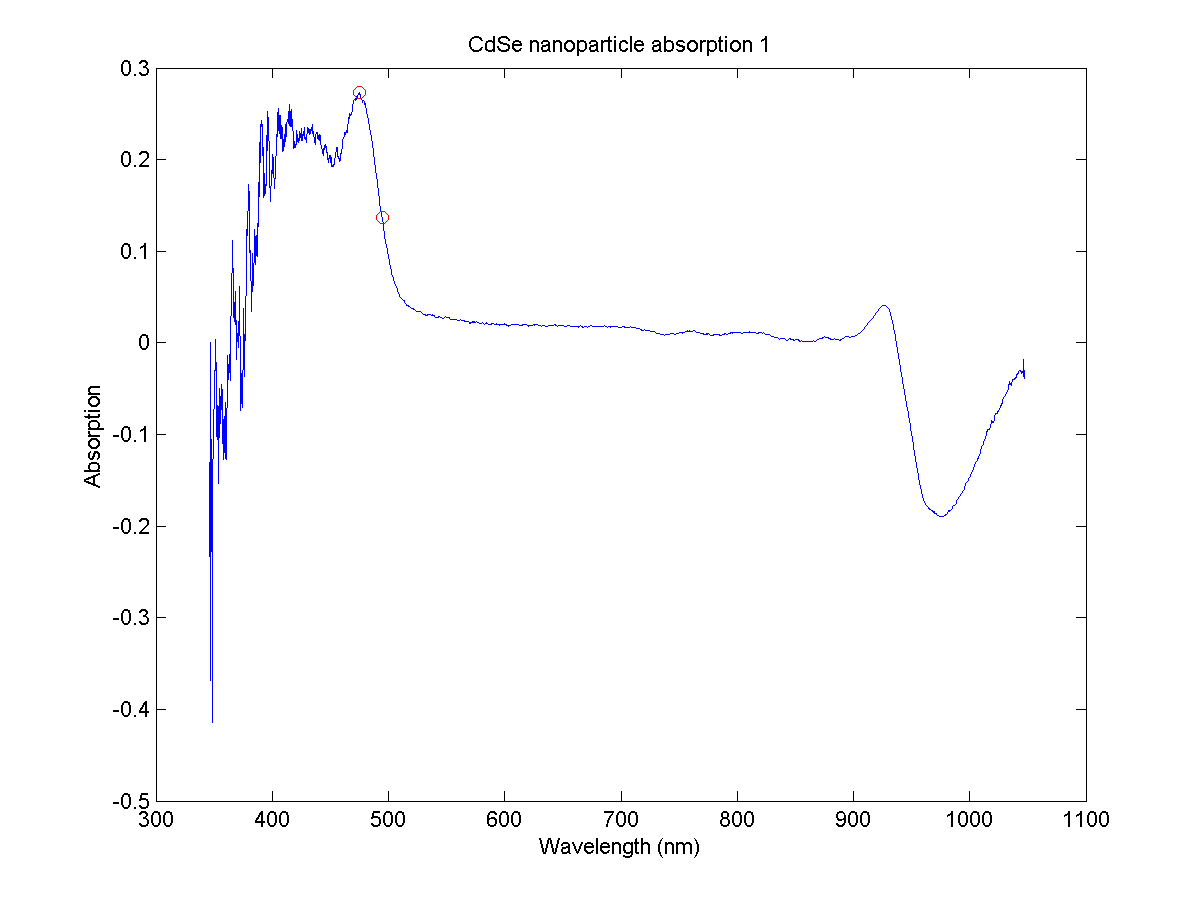
\includegraphics[width=0.8\textwidth]{cdseasp1}
\centering
\caption{Absorption spectrum for the first aliquot of cadmium selenide nanocrystal solution
with peak and FWHM marked.}
\end{figure}

\begin{figure}[H]
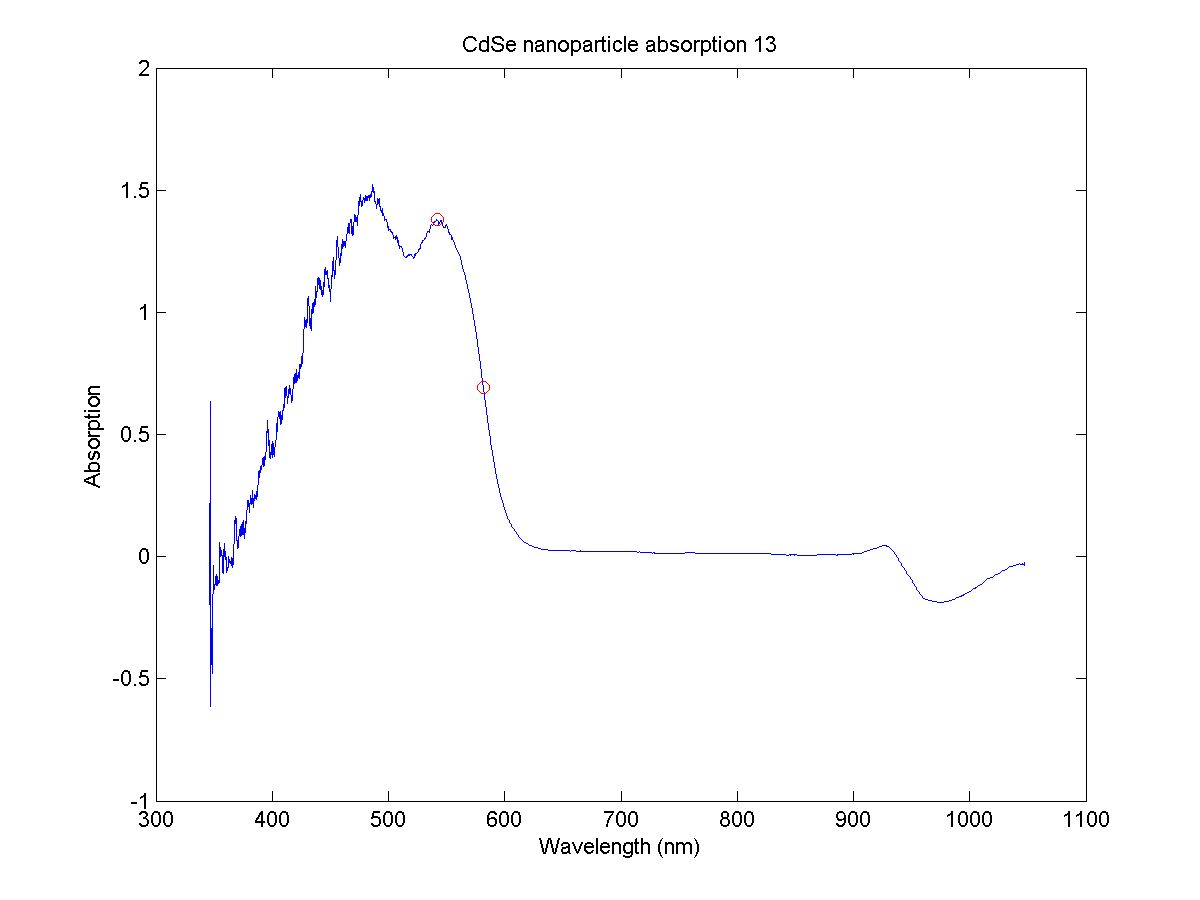
\includegraphics[width=0.8\textwidth]{cdseasp13}
\centering
\caption{Absorption spectrum for the thirteenth aliquot of cadmium selenide nanocrystal 
solution with peak and FWHM marked.}
\end{figure}

The emission spectra for the first and last aliquots of CdSe nanocrystals are included as
Figures 3 and 4. The spectrometer detector was did not cleanly detect wavelengths shorter 
than approximately ultraviolet. The clear absorption band to the right of this noise was 
marked, as best as possible, at peak and FWHM and the corresponding wavelengths were
recorded using MATLAB\footnote{MATLAB script \texttt{zs\textunderscore nanocdse.m}.}.

\begin{figure}[H]
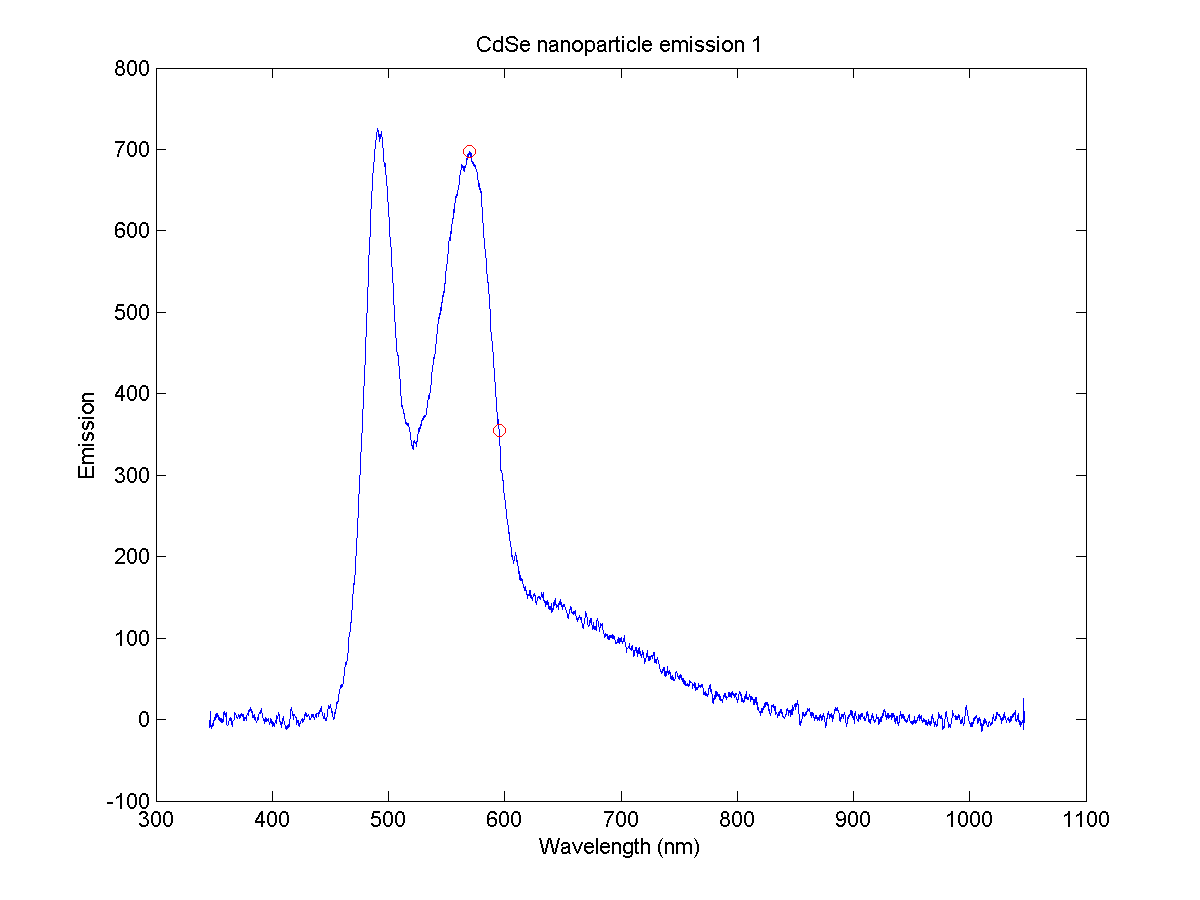
\includegraphics[width=0.8\textwidth]{cdseesp1}
\centering
\caption{Emission spectrum for the first aliquot of cadmium selenide nanocrystal 
solution with peak and FWHM marked.}
\end{figure}

\begin{figure}[H]
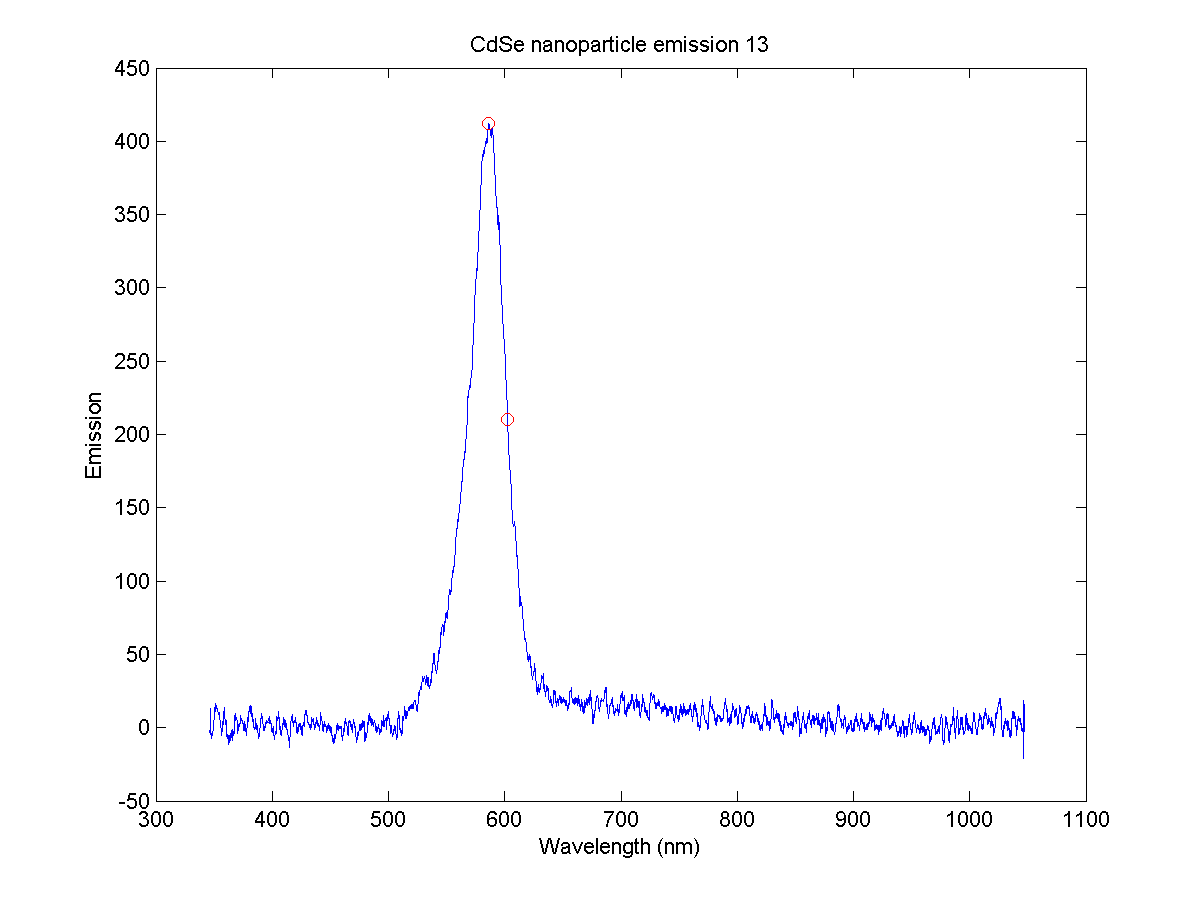
\includegraphics[width=0.8\textwidth]{cdseesp13}
\centering
\caption{Emission spectrum for the thirteenth aliquot of cadmium selenide nanocrystal 
solution with peak and FWHM marked.}
\end{figure}

\subsection{Gold nanoparticles}

The absorption spectra for the original gold nanoparticles is included as
Figure 5\footnote{MATLAB script \texttt{zs\textunderscore nanoau.m}.}. The spectrometer 
detector did not cleanly detect wavelengths shorter than approximately ultraviolet.

\begin{figure}[H]
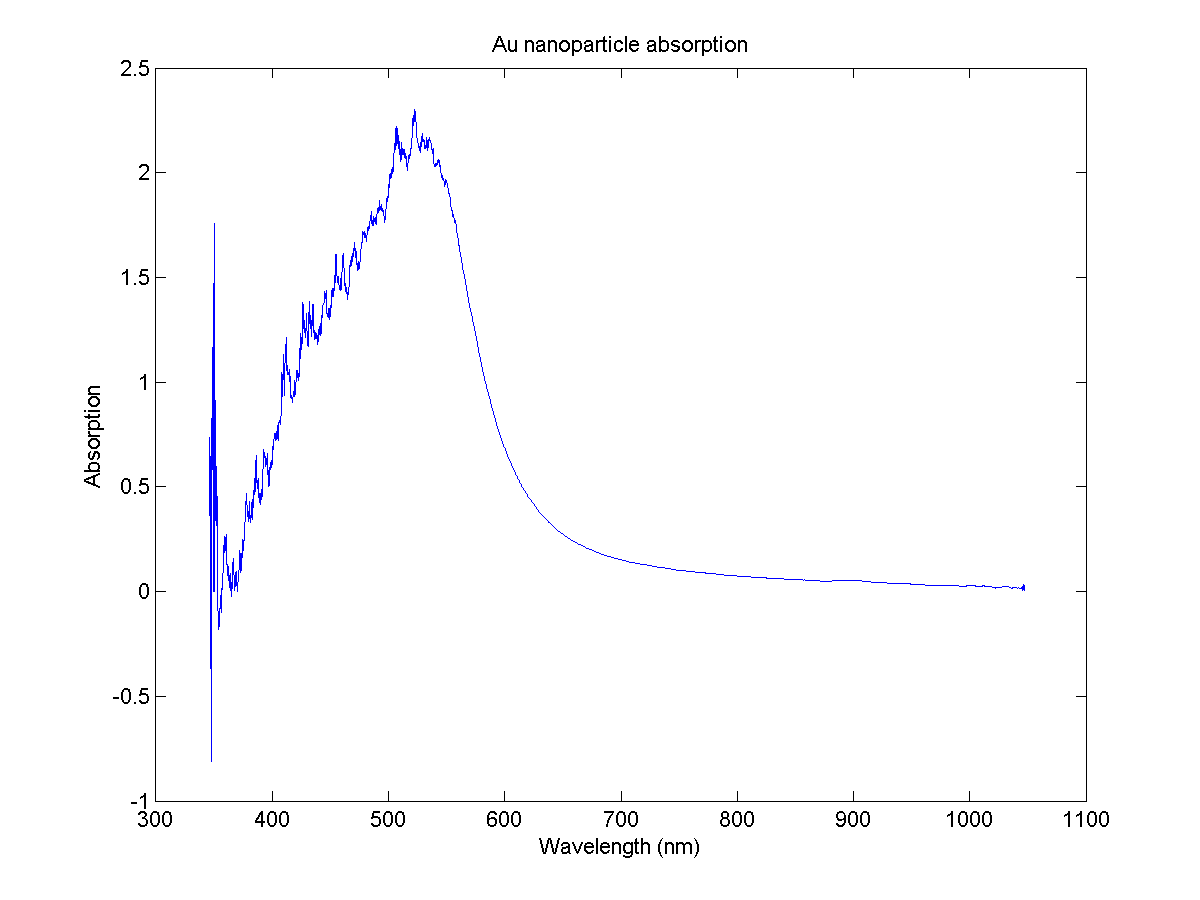
\includegraphics[width=0.8\textwidth]{ausp0}
\centering
\caption{Absorption spectrum of the original gold nanoparticle solution.}
\end{figure}

The first and last absorption spectra taken after the addition of sodium chloride to the
gold nanoparticle solution are included as Figures 6 and 7.

\begin{figure}[H]
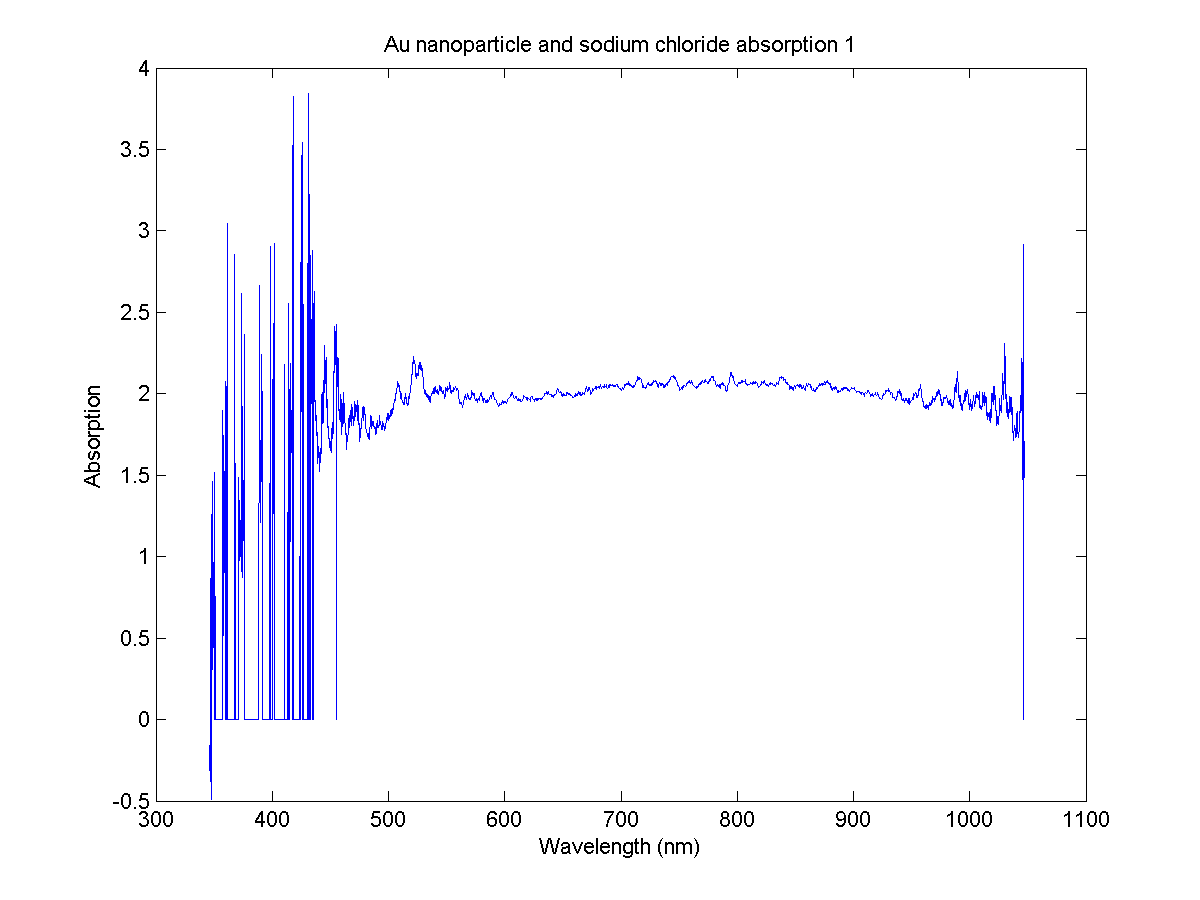
\includegraphics[width=0.8\textwidth]{ausp1}
\centering
\caption{First absorption spectrum of gold nanoparticle solution treated with sodium 
chloride.}
\end{figure}

\begin{figure}[H]
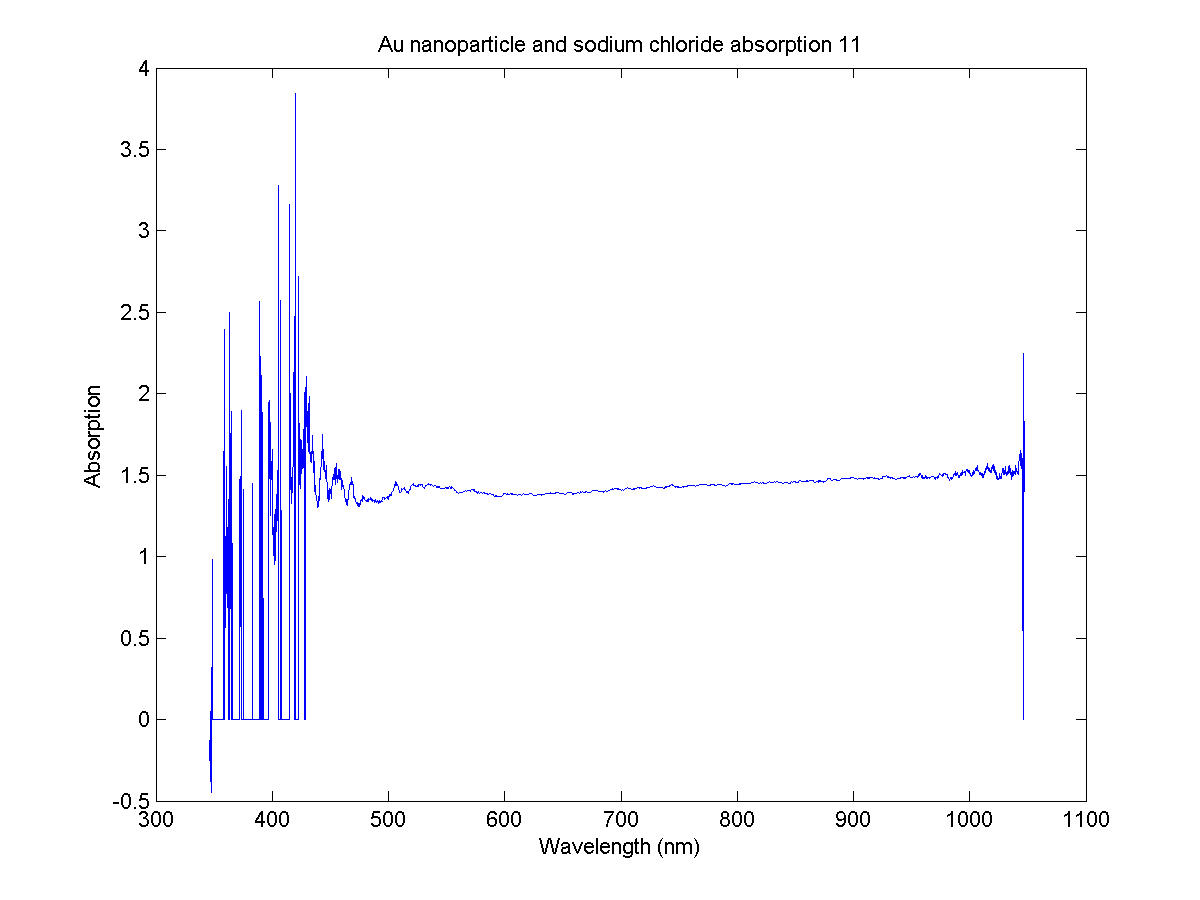
\includegraphics[width=0.8\textwidth]{ausp11}
\centering
\caption{Eleventh absorption spectrum of the gold nanoparticles solution treated with 
sodium chloride.}
\end{figure}

\section{Analysis}

\subsection{Cadmium selenide nanocrystal diameter and color}

The CdSe nanocrystal diameters can be calculated by finding the roots of
Equations (3) and (4), 
which genearate a quadratic equation in $R$, and taking the maximum real part.
Taken from the absorption peak wavelengths, the diameters range from 3.89 nm for the
first aliquout to 4.18 nm for the last aliquot. The wavelengths of the corresponding 
absorption peaks range from 475 nm to 538 nm, corresponding to the absorption of
blue to green light and the transmission of yellow to red light, as expected.

Assuming a Gaussian distribution for the absorption/emission bands of CdSe crystals,
from the estimated full-width-half-maximum (FWHM) plotted above, we calculate a standard 
of deviation, or a variance, of about 44.9 nm.

\subsection{Cadmium Selenide nanocrystal absorption/emission energy shift}

The peak absorption wavelength versus the peak emission wavelength for CdSe nanocrystals
is plotted\footnote{I would plot this with error bars corresponding to the Gaussian variance 
from above, but I don't know how. This would indicated the quality of the coming linear fit.}
in Figure 8 with a superimposed linear fit. The constant term of -299 nm gives 
the energy shift from emission to absorption described above.

\begin{figure}[H]
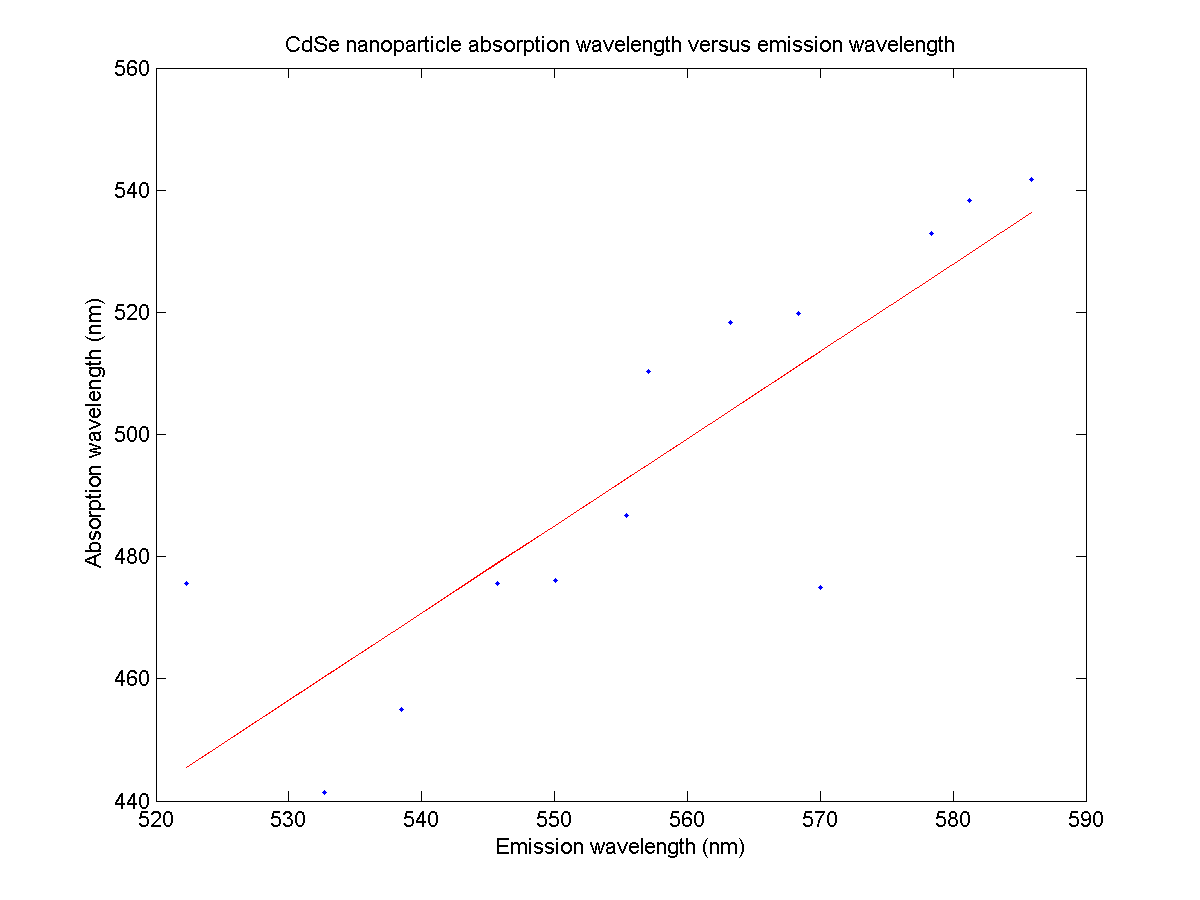
\includegraphics[width=0.8\textwidth]{abvem}
\centering
\caption{Relation between peak absorption and peak emission wavelengths for CdSe
nanocrystals.}
\end{figure}

\subsection{Cadmium Selenide nanocrystal absorption/emission energy shift}

The CdSe nanocrystal diameter versus absorption peak energy is plotted below in Figure 9.
I attempted a least square curve fitting using Equation (1) with initial guesses $n=1$ and
$m_c$ half the rest mass of an electron. Clearly, the shape of the curve and the data
parallel each other, but something has not been accounted for. For one, Equation (1) assumes
only an electron trapped in a box, and not an electron-hole pair.

\begin{figure}[H]
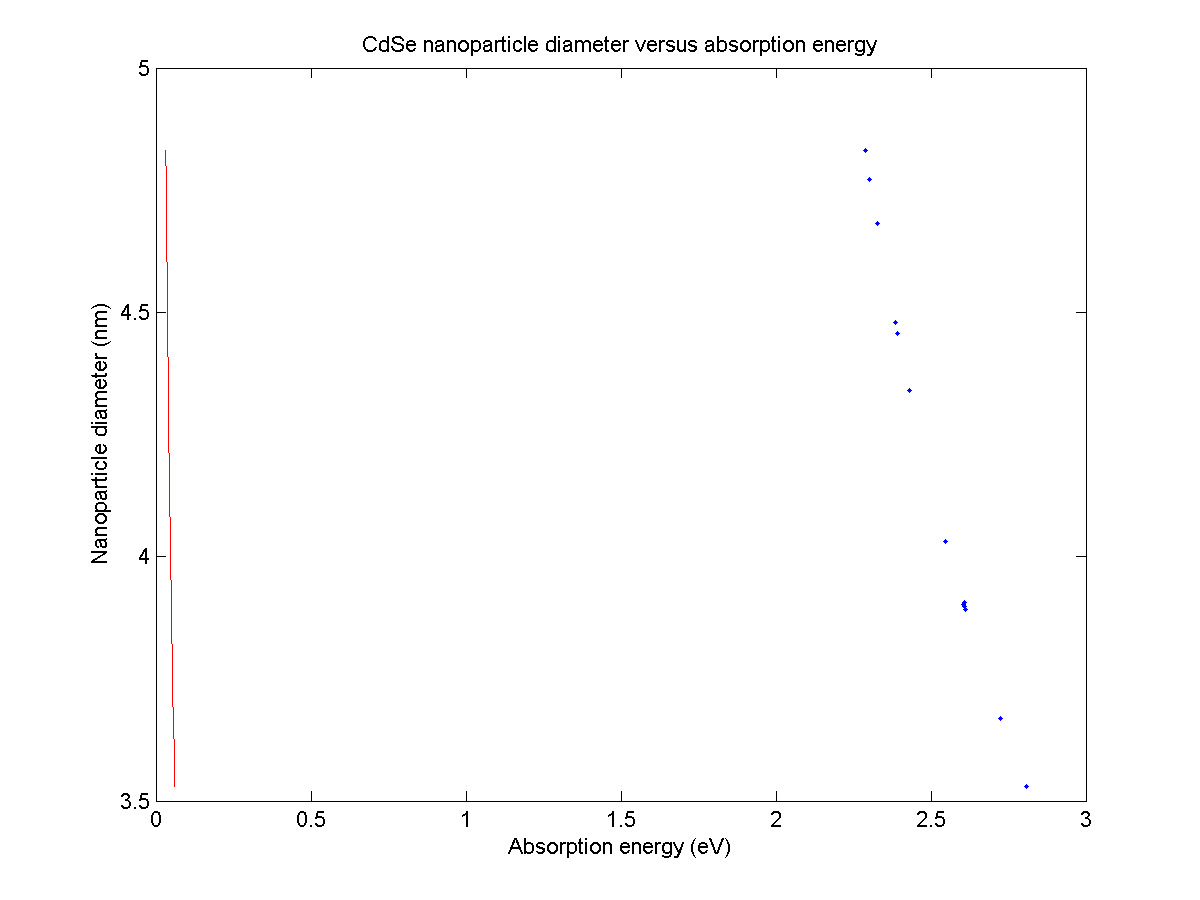
\includegraphics[width=0.8\textwidth]{PiBx}
\centering
\caption{Relation between nanoparticle diameter and absorption energy for CdSe, fit with
a particle in a box equation.}
\end{figure}

\subsection{Simulated absorption spectrum for gold nanoparticles}

The average number of gold atoms in a nanoparticle are given by
\begin{equation}
N=\frac{\pi\rho d^3}{6 M} N_A,
\end{equation}
where $N_A$ is avogardo's constant, $M$ is the atomic mass of gold, $\rho$ is the density
of gold, and $d$ is the average diameter. This can be plugged into the following equation
to give the molar concentration of gold as
\begin{equation}
C_m=\frac{N_T}{N V N_A},
\end{equation}
where $N_T$ is the total number of gold atoms added in the procedure as
HAuCl\textsubscript{4}, and $V$ is the volume of the reaction solution.
The extinction coefficient for the gold nanoparticles at a particular wavelength is
then given by
\begin{equation}
\epsilon(\lambda)=3.0\times10^{-3} \frac{C(R,\lambda)}{\pi R^2}
\frac{1}{C_m 4\cdot2.303 R},
\end{equation}
where $C$ is the absorption cross section computed using Equations (6), (7) and (8).
Using literature\footnote{See procedure.} values for all the constants, most importantly an 
average gold nanoparticle
radius of 6 nm, a simulated gold nanoparticle absorption spectrum\footnote{The orders of
magnitude of the units for the extinction coefficient may be off, but the shape is correct}
 is ploted below in  Figure 10.

\begin{figure}[H]
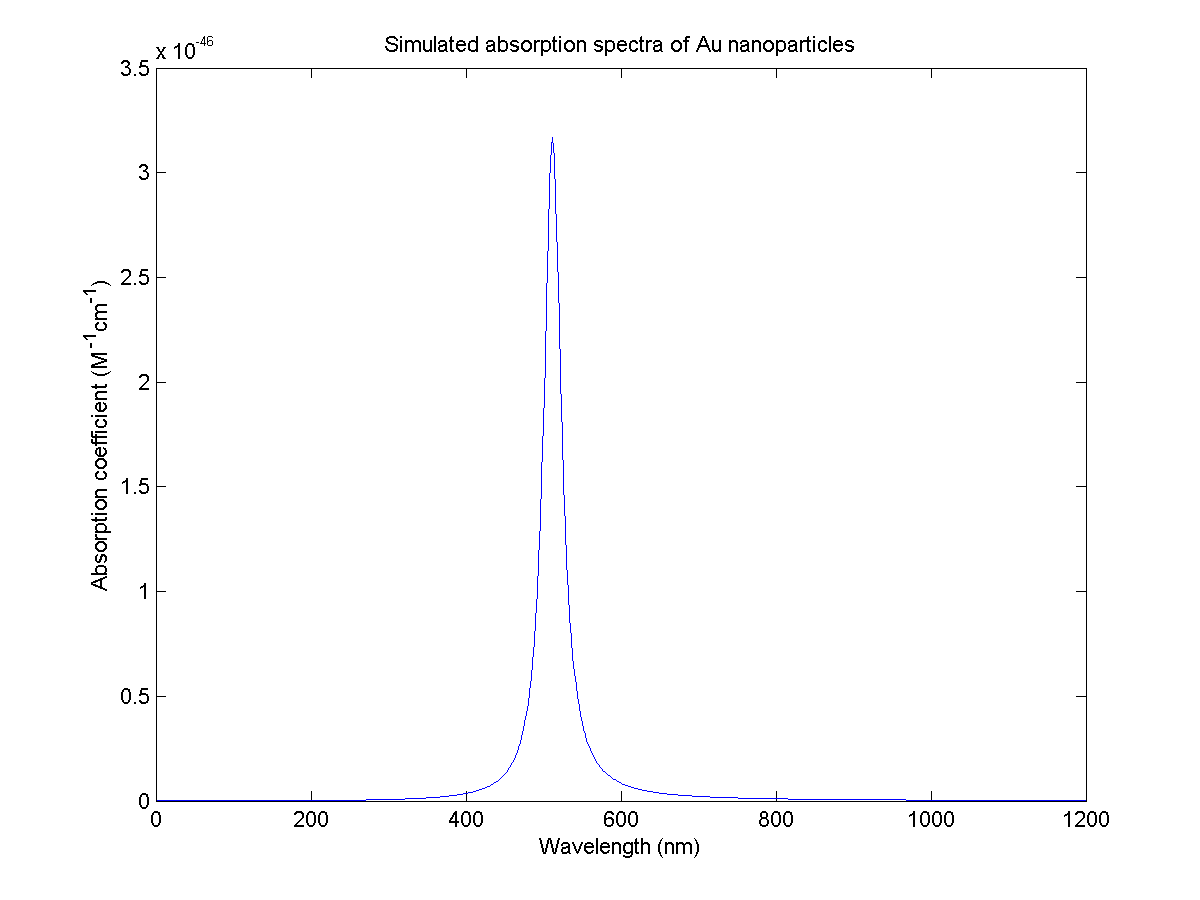
\includegraphics[width=0.8\textwidth]{simauab}
\centering
\caption{Simulated absorption spectra for gold nanoparticles.}
\end{figure}

It is possible to use MATLAB and the above equations to actually fit the extinction coefficient 
spectrum adjusted by the concentration of the solution to the gold nanoparticle spectrum
using some sort of curve fitting. Given the giant size of the equations involved, I have simply 
included the simulated spectrum to give an idea of the theoretical shape.

\section{Discussion}

The citrate ions present in the gold nanoparticle solution forms a hydrophilic shell around 
the neutral metallic nanoparticles. The three carboxylic acid regions of the ion protect
the particle. Addition of sodium chloride drastically increases the cation 
concentration. Aqueous chloride ions are much smaller and more stable 
than giant citrate ions, so the sodium binds to it and draws the 
citrate off of the nanoparticles. I imagine gold, a heavy metal, has a
poor index of refraction on it's own, so it transmits nothing when it
aggregates. Thus, we see almost total absorbance above in Figures 6 and 7.

This lab has presented another view of quantum effects that show visible changes. It has also 
clarified the process by which we quantify and measure said somewhat subjective visual.

%\begin{thebibliography}{9}

%\bibitem{}
%Last, F. I.; Surname, G. N. Title of Article. 
%\textit{Journal Title} [Online] \textbf{Year}, edition, page-page.

%\end{thebibliography}

\end{document}